% !TeX root = ./slides.tex

\documentclass{beamer}
\usepackage{datetime}
\usepackage{mathtools}
\usepackage{amsmath}
\usepackage{amsfonts}
\usepackage{amsthm}
\usepackage{amssymb}

\theoremstyle{plain}
\newtheorem{thm}{Theorem}
\newtheorem{lem}[thm]{Lemma}
\newtheorem{prop}[thm]{Proposition}
\newtheorem*{cor}{Corollary}

\theoremstyle{definition}
\newtheorem{defn}{Definition}
\newtheorem{conj}{Conjecture}
\newtheorem{exmp}{Example}

\theoremstyle{remark}
\newtheorem*{rem}{Remark}
\usepackage{floatrow}

\newenvironment{tzfigure}[1]
{
    \begin{figure}[ht]
        \centering
        #1
        \begin{tikzpicture}
}
{
        \end{tikzpicture}   
    \end{figure}
}

\newenvironment{tzcategory}[1]
{
    \begin{figure}[ht]
        \centering
        #1
        \begin{tikzpicture}[baseline= (a).base]    
}
{
    \end{tikzpicture}   
\end{figure}
}

\newenvironment{subtzcategory}[2]
{
    \begin{subfigure}[ht]{#2}
        \centering
        #1
        \begin{tikzpicture}[baseline= (a).base]    
}
{
    \end{tikzpicture}   
\end{subfigure}
}

\usepackage{graphicx}
\usepackage{caption}
\usepackage{subcaption}
\usepackage{tikz}
\usetikzlibrary{arrows,decorations.markings}
\usetikzlibrary{cd}
\usetikzlibrary{shapes.geometric,fit}
\usetikzlibrary{positioning}
\usepackage{etoolbox}
\listadd{\pc}{\footnotesize$C$}
\listadd{\pc}{\footnotesize$C\sharp$}
\listadd{\pc}{\footnotesize$D$}
\listadd{\pc}{\footnotesize$E\flat$}
\listadd{\pc}{\footnotesize$E$}
\listadd{\pc}{\footnotesize$F$}
\listadd{\pc}{\footnotesize$F\sharp$}
\listadd{\pc}{\footnotesize$G$}
\listadd{\pc}{\footnotesize$G\sharp$}
\listadd{\pc}{\footnotesize$A$}
\listadd{\pc}{\footnotesize$B\flat$}
\listadd{\pc}{\footnotesize$B$}



\usetheme{Singapore}
\usecolortheme{rose}
\usefonttheme{structurebold}
\usebackgroundtemplate{\includegraphics[width=\paperwidth]{./img/background.jpg}}


\setbeamertemplate{navigation symbols}{}
\AtBeginSection[]
{
	\begin{frame}
		\frametitle{Overview}
		\tableofcontents[currentsection]
    \end{frame}
}
\setbeamertemplate{footline}[page number]


\title{EK-nets}
\subtitle{Musical Constraints in Category Theory}
\author{Alice Rixte}
\institute[IRCAM]{ENS Paris-Saclay, IRCAM, CNRS, Sorbonne Université}
\newdate{date}{17}{09}{2020}
\date{\displaydate{date}}


\newcounter{itemcount}

\begin{document}
\begin{frame}
	\titlepage
\end{frame}

\begin{frame}
	\frametitle{Table of contents}
	\tableofcontents
\end{frame}

\section{Introduction}

\subsubsection{Transformational music theory}
\begin{frame}[fragile]
	\frametitle{Transformational music theory}
	\begin{itemize}
		\item Main focus : relations between musical objects
		\item Main tool : T/I group (dihedral group with 12 elements)
	\end{itemize}
	\begin{figure}
		\begin{subfigure}[c]{.27\textwidth}
			\centering
			\setcounter{itemcount}{450}
			\renewcommand*{\do}[1]{
				\filldraw [black](\number\value{itemcount}:3cm)
				circle (1.5pt)
				node[anchor={\number\value{itemcount}-180}]
					{#1\addtocounter{itemcount}{-30}};}
			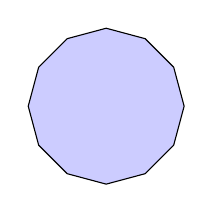
\begin{tikzpicture}[scale=0.33]
				\dolistloop{\pc}
				\draw[fill=blue!20] (90:3cm) -- (60:3cm) -- (30:3cm) -- (0:3cm) --  (330:3cm) -- (300:3cm) -- (270:3cm) -- (240:3cm) -- (210:3cm) -- (180 :3cm) -- (150:3cm) -- (120:3cm) -- cycle;
			\end{tikzpicture}
			\caption{Pitch-classes dodecahedron}
			\label{fig:dode-id}
		\end{subfigure}%
		\hspace{0.2cm}{\color{blue!40}\LARGE$\xRightarrow{T_2}$}\hspace{0cm}%
		\begin{subfigure}[c]{.27\textwidth}
			\centering
			\setcounter{itemcount}{510}
			\renewcommand*{\do}[1]{
				\filldraw [black](\number\value{itemcount}:3cm)
				circle (1.5pt)
				node[anchor={\number\value{itemcount}-180}]
					{#1\addtocounter{itemcount}{-30}};}
			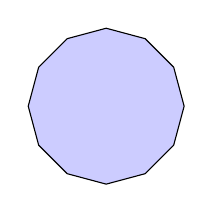
\begin{tikzpicture}[scale=0.33]
				\dolistloop{\pc}
				\draw[fill=blue!20] (90:3cm) -- (60:3cm) -- (30:3cm) -- (0:3cm) --  (330:3cm) -- (300:3cm) -- (270:3cm) -- (240:3cm) -- (210:3cm) -- (180 :3cm) -- (150:3cm) -- (120:3cm) -- cycle;
			\end{tikzpicture}
			\caption{Transposition of 2 semi-tones (Rotation)}
			\label{fig:dode-T2}
		\end{subfigure}%
		\hspace{0.2cm}{\color{purple}\LARGE$\xRightarrow{I_4}$}\hspace{0cm}%
		\begin{subfigure}[c]{.27\textwidth}
			\centering
			\setcounter{itemcount}{510}
			\renewcommand*{\do}[1]{
				\filldraw [black](\number\value{itemcount}:3cm)
				circle (1.5pt)
				node[anchor={\number\value{itemcount}-180}]
					{#1\addtocounter{itemcount}{30}};}
			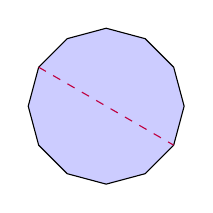
\begin{tikzpicture}[scale=0.33]

				\dolistloop{\pc}
				\draw[fill=blue!20] (90:3cm) -- (60:3cm) -- (30:3cm) -- (0:3cm) --  (330:3cm) -- (300:3cm) -- (270:3cm) -- (240:3cm) -- (210:3cm) -- (180 :3cm) -- (150:3cm) -- (120:3cm) -- cycle;
				\draw[purple,dashed] (150:3cm) -- (330:3cm);
			\end{tikzpicture}
			\caption{$4^{th}$ inversion  (Symmetry)}
			\label{fig:dode-I4}
		\end{subfigure}%
		\caption{Transpositions and inversions in a dodecahedron}
		\label{fig:dode-TI}
	\end{figure}

\end{frame}

\subsubsection{K-nets : using the T/I group}


\begin{frame}[fragile]
	\frametitle{K-nets : using the T/I group}
	\begin{columns}
		\begin{column}{0.4\textwidth}
			\begin{column}{0.85\textwidth}

				\begin{figure}
					\centering

					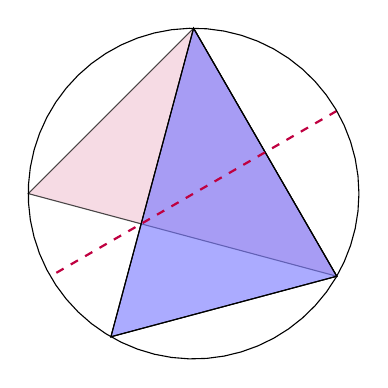
\begin{tikzpicture}[scale=0.7]
						\setcounter{itemcount}{450}
						\renewcommand*{\do}[1]{
							\filldraw [black](\number\value{itemcount}:3cm)
							circle (1.5pt)
							node[anchor={\number\value{itemcount}-180}]
								{#1\addtocounter{itemcount}{-30}};}

						\dolistloop{\pc}
						\draw[fill=purple!20,opacity=0.7] (90:3cm) -- (330:3cm) -- (180:3cm) -- cycle;
						\draw[fill=blue!55, fill opacity=0.6] (90:3cm) -- (330:3cm) -- (240:3cm) -- cycle;
						\draw (90:3cm) -- (330:3cm) -- (240:3cm) -- cycle;
						\draw [dashed, thick, purple, opacity=1] (30:3cm) -- (210:3cm);
						\draw [domain=0:360,samples=60] plot ({3*cos(\x)}, {3*sin(\x)});

					\end{tikzpicture}
					\caption{The $I_4$ inversion on the C major chord}
					\label{fig:Rtransf}
				\end{figure}
			\end{column}
			
		\end{column}
		\pause
		\begin{column}{0.5\textwidth}
			\begin{equation*}
				\left\{ \begin{aligned}
					T_i & \rightarrow T_{11i}   & = T_{-i}     \\
					I_j & \rightarrow I_{11j+4} & = T_{-j + 4} \\
				\end{aligned} \right.
			\end{equation*}

			\vspace{0cm}

			\begin{figure}[ht]

				\begin{subfigure}{.46\textwidth}
					\centering
					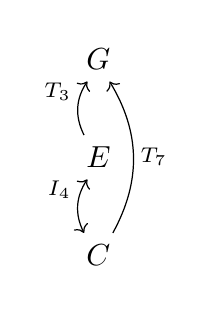
\begin{tikzpicture}
						% https://tikzcd.yichuanshen.de/#N4Igdg9gJgpgziAXAbVABwnAlgFyxMJZABgBoAmAXVJADcBDAGwFcYkQBhEAX1PU1z5CKMgEZqdJq3YBRHnxAZseAkTLEJDFm0QgA4jwkwoAc3hFQAMwBOEALZIyIHBCSiaAIxhgoSAMxOWtK6ACoA+gAs8la2Dojuzq6I5J7evogBNEE6IOF+0SA29o40LkgpIF4+SAC0mc70WIzskGBsNHAAFliWOCUgjPRejAAKAirCINZYJp19WVI5AJJhAOyG3EA
						\node[scale=1.1] (a) at (0,0){
							\begin{tikzcd}
								G\\
								E \arrow[u, "T_3", bend left]\\
								C \arrow[u, "I_4",leftrightarrow, bend left]
								\arrow[uu, "T_7"',  bend right]
							\end{tikzcd}
						};
					\end{tikzpicture}
					\caption{C K-net}
					\label{fig:KCmajor}
				\end{subfigure}%
				%\hspace{-0.2cm}%
				{\Large$\xRightarrow{\text%
						{\scriptsize $F\big< 11,4 \big>$}}$}%
				%\hspace{-0.2cm}%
				\begin{subfigure}{.50\textwidth}
					\centering

					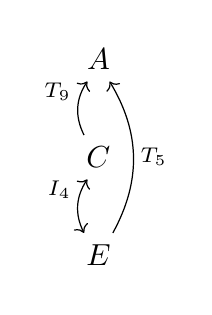
\begin{tikzpicture}

						% https://tikzcd.yichuanshen.de/#N4Igdg9gJgpgziAXAbVABwnAlgFyxMJZABgBoAmAXVJADcBDAGwFcYkQBhEAX1PU1z5CKMgEZqdJq3YBRHnxAZseAkTLEJDFm0QgA4jwkwoAc3hFQAMwBOEALZIyIHBCSiaAIxhgoSAMxOWtK6ACoA+gAs8la2Dojuzq6I5J7evogBNEE6IOF+0SA29o40LkgpIF4+SAC0mc70WIzskGBsNHAAFliWOCUgjPRejAAKAirCINZYJp19WVI5AJJhAOyG3EA
						\node[scale=1.1] (a) at (0,0){
							\begin{tikzcd}
								A \\
								C \arrow[u, "T_9", bend left]\\
								E \arrow[u, "I_4",leftrightarrow, bend left]
								\arrow[uu, "T_5"', bend right]
							\end{tikzcd}
						};
					\end{tikzpicture}
					\caption{Am K-net}
					\label{fig:KAminor}
				\end{subfigure}
				\caption{Isography between C and Am}
				\label{fig:Kisography}
			\end{figure}
		\end{column}
	\end{columns}
\end{frame}

\subsubsection{K-nets and T/I automorphisms}
\begin{frame}[fragile]
	\frametitle{K-nets and T/I automorphisms}
\end{frame}


\section{EK-nets}

\subsubsection{EK-nets presentation}
\begin{frame}
	\frametitle{EK-nets presentation}
\end{frame}

\subsubsection{Structural constraints}
\begin{frame}
	\frametitle{Structural constraints}
\end{frame}

\subsubsection{Relational Constraints}
\begin{frame}
	\frametitle{Relational constraints}
\end{frame}

\subsubsection{Pitch-classes as structural constraintsn}
\begin{frame}
	\frametitle{Pitch-classes as structural constraints}
\end{frame}

\subsubsection{ETranspositions as relational constraints}
\begin{frame}
	\frametitle{Transpositions as relational constraints}
\end{frame}





\section{Perspectives}
\subsubsection{EK-nets as relational constraints}
\begin{frame}
	\frametitle{K-nets as relational constraints}
\end{frame}

\subsubsection{Forte's interval vector as constraints}
\begin{frame}
	\frametitle{Forte's interval vector as constraints}
\end{frame}

\subsubsection{Compositionnal tools}
\begin{frame}
	\frametitle{Compositionnal tools}
\end{frame}

\subsubsection{Live possibilities}
\begin{frame}
	\frametitle{Live possibilities}
\end{frame}


\section{Conclusion}
\end{document}
